
\subsubsection{Einf\"uhrung}
Damit der User die M\"oglichkeit hat die aufgezeichneten Videos abzuspielen, wird ein Webinterface bereitgestellt. Dieses informiert den User zudem \"uber das Projekt und seinen Aufbau. Auch die Eintr\"age aus der Datenbank, der bereits gel\"oschten Videos k\"onnen im Webinterface angezeigt werden.\\ 
\\
Das Webinterface ist \"uber einen Apache Webserver auf dem Raspberry PI aus dem lokalen Netzwerk erreichbar. 

\subsubsection{PHP Skript}
Um auf die MySQL\footnote{\hyperlink{http://www.mysql.com/}{http://www.mysql.com/}} Datenbank mit den Daten der Aufzeichnungen zuzugreifen wird ein Serverseitiges PHP-Skript\footnote{\hyperlink{https://secure.php.net/}{https://secure.php.net}} verwendet. Dieses verbindet sich auf den Datenbank Server und stellt SQL-Anfangen\footnote{\hyperlink{http://www.iso.org/iso/catalogue_detail.htm?csnumber=53682}{http://www.iso.org/iso/catalogue_detail.htm?csnumber=53682}} an den Server, um die ben\"otigten Daten, wie Video-Path, Datum der Aufzeichnung und ID zu erhalten.
Anschlie\ss end wird HTML\footnote{\hyperlink{https://www.w3.org/TR/2014/REC-html5-20141028/}{https://www.w3.org/TR/2014/REC-html5-20141028}}
generiert, das die Daten in einer Tabelle darstellt. Durch Aufruf des PHP-Skripts durch einen Browser, wird das PHP-Skript vom Server kompiliert und ausgef\"uhrt, sodass das generierte HTML ausgegeben wird.\\
\\
\begin{figure}[htb]
  \centering
    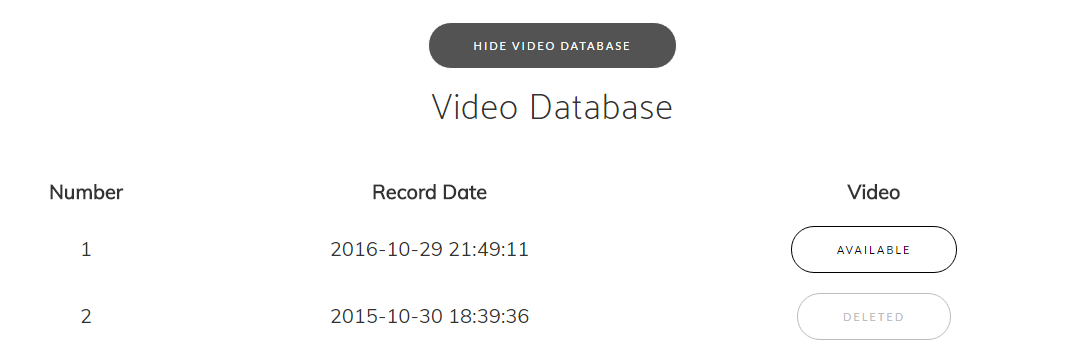
\includegraphics[width=1.0\textwidth]{images/phptable}
    \caption{Ausgabe der Video Database im Browser.}
\end{figure}
\\
Die Eintr\"age innerhalb der Tabelle, in der Spalte Video verweisen jeweils auf das Video, das unterhalb der Tabelle in die Seite eingebettet ist. So ist es dem User m\"oglich sich einen \"Uberblick \"uber die vorhandenen Aufzeichnungen zu verschaffen und beim Klick auf den Available-Button in der Tabelle zum Video zu gelangen.
In der Tabelle werden zudem auch die Eintr\"age von Aufzeichnungen angezeigt, bei denen das Video-File bereits die festgelegte Zeit \"uberschritten hat und gel\"oscht wurde. \\
\\
\begin{figure}[htb]
  \centering
    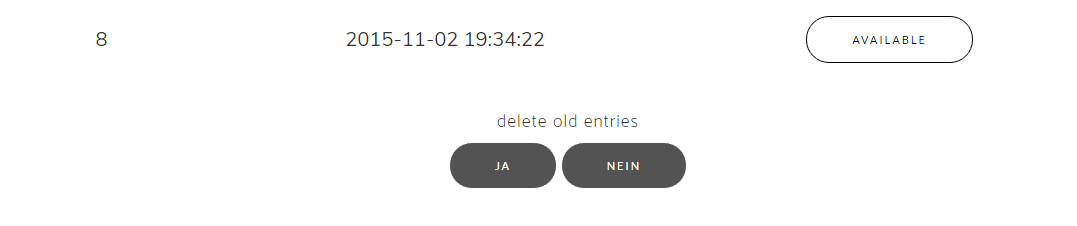
\includegraphics[width=1.0\textwidth]{images/phpdel}
    \caption{Button zum L\"oschen der Eintr\"age}
\end{figure}
\\
Wenn diese Eintr\"age nicht mehr ben\"otigt werden, kann der User unterhalb der Tabelle mit Klick auf einen Button alle alten Eintr\"age aus der Datenbank l\"oschen lassen. Hierbei wird f\"ur jeden Eintrag, der kein VideoPath Eintrag in der Datenbank besitzt, ein SQL Befehl von dem PHP-Skript an den MySQL-Server gesendet, der diesen Eintrag l\"oscht.\\
\begin{figure}[htb]
  \centering
    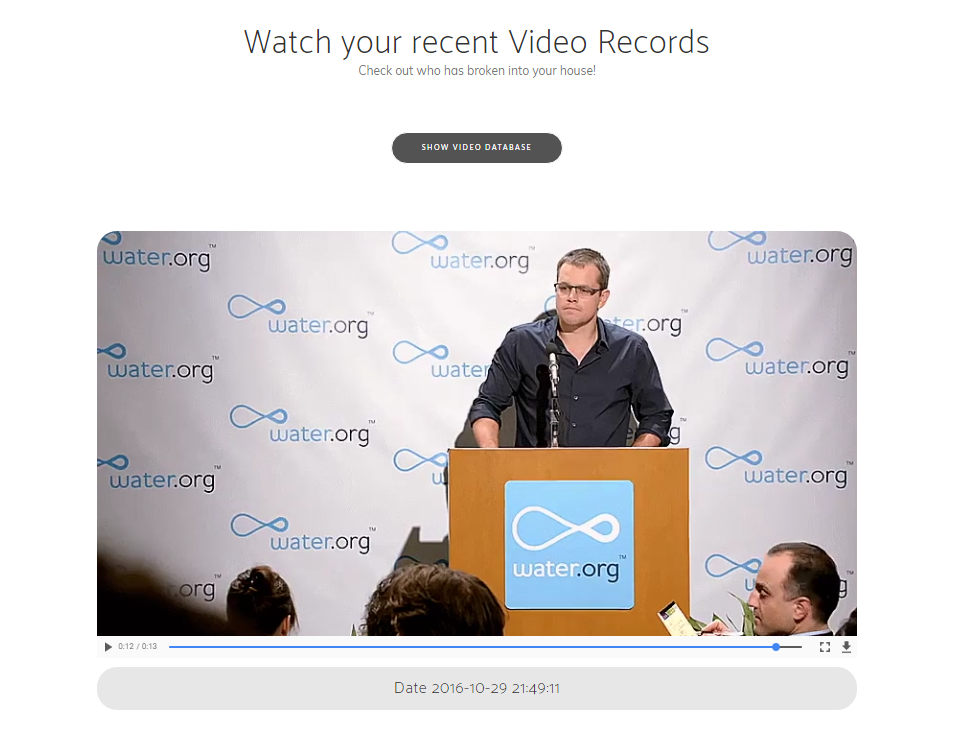
\includegraphics[width=1.0\textwidth]{images/video}
    \caption{Eingebettetes Video}
\end{figure}
\\
Unter der Tabelle der Video Database werden alle aufgezeichneten Videos mit Datum aufgelistet. Dabei fordert das PHP-Skript alle Eintr\"age aus der Records Tabelle an und iteriert in einer Schleife durch jeden Eintrag. Bei allen Eintr\"agen mit VideoPath Eintrag wird eine HTML Section\footnote{\hyperlink{https://developer.mozilla.org/de/docs/Web/HTML/Element/section}{https://developer.mozilla.org/de/docs/Web/HTML/Element/section}} generiert, in die das Video mittels Video-Tag eingebettet wird. Durch das Anlegen des Section-Tags ist es sp\"ater m\"oglich, den User zum entsprechenden Video zu schicken, nachdem er auf einen Eintrag in der Video Database Tabelle geklickt hat.\\


\begin{lstlisting}[language=PHP,caption={Auszug aus dem PHP-Skript (Videos auflisten)},numbers=left,frame=lrbt]
if ($result->num_rows > 0) 
{
    while($row = $result->fetch_assoc()) 
    {
        $i++;
		if($row["VideoPath"] != null)
		{	
			echo "<section id=\"" ."$i". "\">";			
			echo "<h2>";
			echo "
            <video width=\"100%\" height=\"auto\" controls>
                <source src=\" ". $row["VideoPath"]."\" type=\"video/mp4\">
                Your browser does not support the video tag.
            </video>";	
			echo "<h3>Date " . $row["RecordDateTime"]. "</h3><br><br>";		
			echo "</section>";
		}
    }
} 
\end{lstlisting}

\subsubsection{Frontend}

F\"ur das Webinterface wurde eine f\"ur das Projekt angepasste Version des Bootstrap\footnote{\hyperlink{http://getbootstrap.com/}{http://getbootstrap.com}} Theme New-Age\footnote{\hyperlink{https://startbootstrap.com/template-overviews/new-age/}{https://startbootstrap.com/template-overviews/new-age}} verwendet. Das HTML/CSS\footnote{\hyperlink{https://www.w3.org/TR/CSS22/}{https://www.w3.org/TR/CSS22}}/JS\footnote{\hyperlink{https://developer.mozilla.org/de/docs/Web/JavaScript}{https://developer.mozilla.org/de/docs/Web/JavaScript}} Framework Bootstrap besteht nur aus Clientseitigem Code und bietet daher wenig Fl\"ache f\"ur Angreifer. Es ben\"otigt wenig Ressourcen und verwendet den aktuellen Webstandard HTML 5.\\
\\
Die Anforderung war, dass das Frontend der Seite auf aktuellem HTML 5 aufbaut, light-weight\footnote{\hyperlink{http://whatis.techtarget.com/definition/lightweight}{http://whatis.techtarget.com/definition/lightweight}} ist d.h. wenig Server Ressourcen belegt und Angreifern wenig Spielraum l\"asst. Zudem muss sich das PHP-Skript einbetten lassen. Ein CMS\footnote{\hyperlink{https://de.wikipedia.org/wiki/Content-Management-System}{https://de.wikipedia.org/wiki/Content-Management-System}} wie z.B. Joomla\footnote{\hyperlink{https://www.joomla.org}{https://www.joomla.org}} ist hier zu anf\"allig f\"ur Angriffe\footnote{\hyperlink{https://www.heise.de/security/meldung/Jetzt-patchen-Angriffe-auf-ueber-30-000-Joomla-Webseiten-3454720.html}{https://www.heise.de/security/meldung/Jetzt-patchen-Angriffe-auf-ueber-30-000-Joomla-Webseiten-3454720.html}} und belegt unn\"otig Ressourcen. Daher wurde das light-weight CMS GRAV\footnote{\hyperlink{https://getgrav.org/}{https://getgrav.org}} in Betracht gezogen, das jedoch keine Einbindungen von PHP-Skripten unterst\"utzt. \\

\paragraph{Aufbau der Website}


\begin{figure}[htb]
  \centering
    
\includegraphics[width=1.0\textwidth]{images/webmenu}
    \caption{Men\"u des Webinterfaces}
\end{figure}

\begin{description}
   \begin{itemize}
      \item Intro mit allgemeinen Informationen.
      \item Download des Projekts von Github.
      \item Anzeige der Videoaufzeichnungen mittels PHP-Skript.
      \item Kontakt.
   \end{itemize}
\end{description}
\begin{figure}[htb]
  \centering
    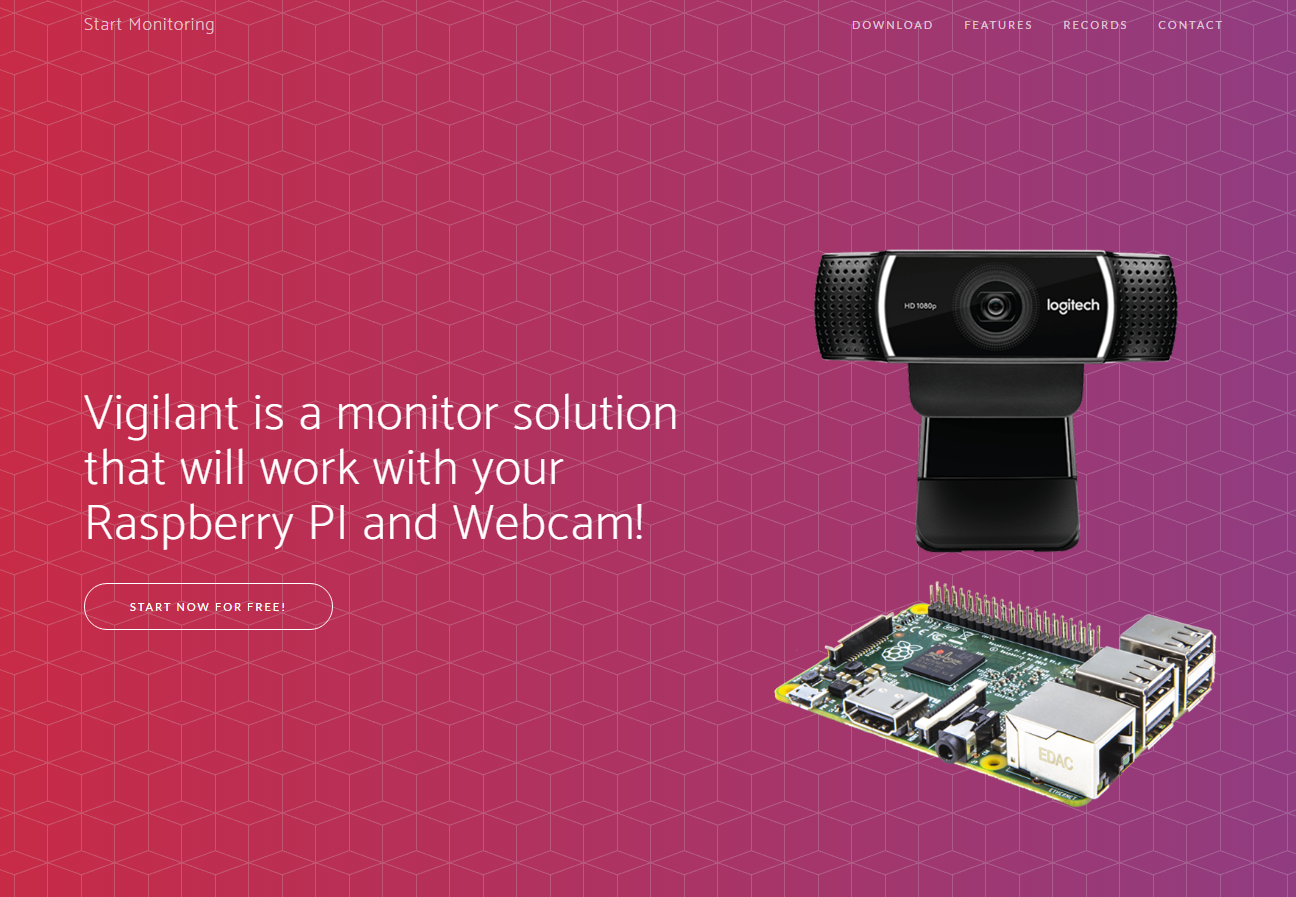
\includegraphics[width=1.0\textwidth]{images/vigilant}
    \caption{Intro der Projektseite}
\end{figure}
Eine exemplarische Implementierung findet man unter  {\href{https://www.schukies.io/vigilant}{https://schukies.io/vigilant}}








